% paper.tex -- Main IEEE-style journal paper
% Active Circuit Discovery: EFE-Guided Mechanistic Interpretability in LLMs
% Compiled with: pdflatex -> bibtex -> pdflatex -> pdflatex

\documentclass[journal]{IEEEtran}

% --- Core packages ---
\usepackage[T1]{fontenc}
\usepackage[utf8]{inputenc}
\usepackage{lmodern}
\usepackage{microtype}

% --- Math ---
\usepackage{amsmath,amssymb,amsthm}
\usepackage{bm}
\usepackage{mathtools}

% --- Graphics and figures ---
\usepackage{graphicx}
\usepackage{tikz}
\usepackage{pgfplots}
\usetikzlibrary{shapes.geometric, arrows.meta, positioning, fit,
                decorations.pathreplacing, calc, backgrounds,
                matrix, chains, scopes}
\pgfplotsset{compat=1.18}

% --- Tables ---
\usepackage{booktabs}
\usepackage{tabularx}
\usepackage{multirow}
\usepackage{array}
\usepackage{makecell}

% --- Algorithms ---
\usepackage{algorithm}
\usepackage{algpseudocode}
\algnewcommand\algorithmicinput{\textbf{Input:}}
\algnewcommand\algorithmicoutput{\textbf{Output:}}
\algnewcommand\Input{\item[\algorithmicinput]}
\algnewcommand\Output{\item[\algorithmicoutput]}

% --- Hyperlinks and cross-refs ---
\usepackage[hyphens]{url}
\usepackage[colorlinks=true, linkcolor=blue, citecolor=blue, urlcolor=blue]{hyperref}
\usepackage{cleveref}

% --- Code listings ---
\usepackage{listings}
\lstset{
  basicstyle=\small\ttfamily,
  keywordstyle=\bfseries,
  commentstyle=\itshape,
  frame=single,
  breaklines=true,
  captionpos=b,
  numbers=left,
  numberstyle=\tiny,
  language=Python
}

% --- Bibliography ---
\usepackage{cite}

% --- Theorem environments ---
\newtheorem{definition}{Definition}
\newtheorem{proposition}{Proposition}
\newtheorem{theorem}{Theorem}

% --- Custom commands ---
\newcommand{\EFE}{\ensuremath{\mathcal{G}}}
\newcommand{\FE}{\ensuremath{\mathcal{F}}}
\newcommand{\KL}[2]{\ensuremath{D_{\mathrm{KL}}\!\left(#1 \,\|\, #2\right)}}
\newcommand{\E}[1]{\ensuremath{\mathbb{E}\!\left[#1\right]}}
\newcommand{\softmax}{\ensuremath{\operatorname{softmax}}}
\newcommand{\Attn}{\ensuremath{\operatorname{Attn}}}
\newcommand{\MLP}{\ensuremath{\operatorname{MLP}}}
\newcommand{\abs}[1]{\ensuremath{\left|#1\right|}}
\newcommand{\norm}[1]{\ensuremath{\left\|#1\right\|}}
\newcommand{\vect}[1]{\ensuremath{\bm{#1}}}
\newcommand{\mat}[1]{\ensuremath{\mathbf{#1}}}
\newcommand{\ACDC}{\textsc{acdc}}
\newcommand{\EAP}{\textsc{eap}}
\newcommand{\ACD}{\textsc{acd}}
\newcommand{\pymdp}{\texttt{pymdp}}

% --- Document metadata ---
\begin{document}

\title{Active Circuit Discovery: Uncertainty-Weighted Feature Selection\\
       for Mechanistic Interpretability}

\author{Sharath~Sathish%
\thanks{S.~Sathish is with the Department of Computer Science,
University of York, York, UK.
This work was conducted as part of the MSc Computer Science
research programme.  Manuscript received February 2026.}%
}

\markboth{IEEE Transactions on Neural Networks and Learning Systems,~Vol.~XX,
No.~X, 2026}%
{Sathish: Active Circuit Discovery}

\maketitle

% =====================================================================
\begin{abstract}
Mechanistic interpretability seeks to reverse-engineer the computational
circuits within large language models, yet current methods rely on
exhaustive or heuristic search over exponentially many feature
interactions. This paper introduces \emph{Active Circuit Discovery}
(\ACD{}), a framework that combines attribution graph analysis with
active inference for efficient circuit discovery. The framework
integrates Anthropic's \texttt{circuit-tracer} library as the
attribution graph backend, using Edge Attribution Patching with
transcoders to identify active transcoder features per prompt.
A POMDP agent, implemented with \texttt{pymdp}, maintains a
multi-factor generative model of feature importance, layer role,
and causal influence, and selects interventions by minimising
Expected Free Energy. The agent learns its observation model online
through Dirichlet parameter updates, enabling principled
exploration of the circuit structure.
The framework is evaluated on two architectures, Gemma-2-2B (26 layers)
and Llama-3.2-1B (16 layers), across four settings: Indirect Object
Identification (IOI), multi-step reasoning, feature steering, and a
multi-domain benchmark spanning geography, mathematics, science, logic,
and history. With a budget of 20 interventions per prompt, the POMDP
agent identifies causally important features more efficiently than
random selection, though a simpler bandit heuristic achieves higher
immediate oracle efficiency at the cost of principled uncertainty
quantification.
Feature steering confirms causal controllability: scaling individual
features at $10\times$ activation changes predictions for a subset of
tested features.
Multi-domain analysis reveals task-dependent circuit structure: IOI
circuits concentrate in late layers, while reasoning and scientific
knowledge recruit early and middle layers.
Code, notebooks, and experiment results are publicly available.

\end{abstract}

\begin{IEEEkeywords}
mechanistic interpretability, active inference, circuit discovery,
transcoders, transformer language models, Gemma, Llama,
uncertainty-weighted exploration, causal circuit analysis, attribution graphs
\end{IEEEkeywords}

% =====================================================================
\section{Introduction}
\label{sec:intro}
% ---- introduction.tex ----

The rapid growth in the scale and deployment of large language models (LLMs) has
intensified the need for principled methods to audit, explain, and predict their
behaviour~\cite{Bereska2024}. Mechanistic interpretability pursues this goal by
reverse-engineering the internal computations of trained models into human-legible
circuits~\cite{Olah2020,Elhage2021}. A circuit, in this context, denotes the minimal
subgraph of model components~-- attention heads, MLP neurons, or SAE features~-- whose
activations are jointly necessary and sufficient to reproduce a specific model
behaviour on a given family of inputs~\cite{Cammarata2020,Wang2022}.

Circuit analysis has produced landmark findings: Wang et al.\ identified a
fourteen-head circuit mediating Indirect Object Identification (IOI) in GPT-2
Small~\cite{Wang2022}; Hanna et al.\ localised a circuit for numerical
greater-than comparisons~\cite{Hanna2023}; and Nanda et al.\ traced the emergence of
modular arithmetic generalisation through a Fourier-space circuit during
grokking~\cite{Nanda2023Grokking}. Each of these studies required thousands of
manually guided interventions, prompting interest in automation~\cite{Conmy2023,Syed2023}.

Automated Circuit Discovery (\ACDC)~\cite{Conmy2023} generalises the activation
patching methodology of Wang et al.\ to a greedy graph-pruning algorithm that
systematically tests every edge in the computational graph. Although \ACDC\ achieves
strong fidelity on the IOI task, the number of interventions scales as $O(E)$ in the
number of graph edges, which for deep transformer models reaches the tens of
thousands. Edge Attribution Patching (\EAP)~\cite{Syed2023} reduces this cost by
approximating patch effects with integrated gradients, yet it trades correctness for
efficiency and may miss higher-order interactions. Neither method incorporates
uncertainty about the circuit structure or adapts its search strategy based on what
has already been discovered.

Active Inference is a normative framework for perception and action in biological
agents that unifies perception, learning, and planning under a single objective: the
minimisation of variational free energy (equivalently, the maximisation of model
evidence)~\cite{Friston2010,Parr2022}. When extended to planning, the framework
introduces the Expected Free Energy (\EFE), which decomposes into an epistemic term
(expected information gain about hidden states) and a pragmatic term (expected
alignment with preferences)~\cite{Friston2015,DaCosta2020}. Crucially, \EFE\
minimisation naturally trades off exploration and exploitation: an agent selects
actions that resolve uncertainty about the world while pursuing desired outcomes.

This work proposes that circuit discovery is precisely the kind of problem for which
\EFE\ minimisation is appropriate. The ``world'' is the causal graph of an LLM; the
``actions'' are ablation and activation-patching interventions; the ``hidden states''
are the identities and importances of circuit-critical features; and the ``preference''
is the rapid identification of a faithful, minimal circuit. An Active Inference agent
that maintains a belief distribution over candidate circuit components and selects
interventions to maximally resolve that uncertainty will, in theory, identify circuits
with fewer total interventions than either random or gradient-ranked selection.

The contributions of this paper are as follows.

\textbf{(C1) Theoretical framing.} A formal mapping is established between
active inference and circuit discovery, showing how transcoder features correspond
to candidate circuit components, how ablation effects correspond to observations,
and how uncertainty-weighted scoring implements the exploration--exploitation
trade-off analogous to Expected Free Energy minimisation.

\textbf{(C2) Framework implementation.} The Active Circuit Discovery (\ACD)
framework is implemented in Python, integrating Anthropic's
\texttt{circuit-tracer}~\cite{Anthropic2025CT,Ameisen2025} for Edge Attribution Patching
with GemmaScope transcoders and the \texttt{feature\_intervention} API for
causally correct transcoder-level interventions on Gemma-2-2B.

\textbf{(C3) Validated evaluation.} Three research questions are defined with
quantified targets and evaluated on two benchmarks (IOI, multi-step reasoning)
with three baselines (random, greedy, oracle), all using real model activations.
The \ACD{} selector achieves 36--44\% improvement over random selection and
74--78\% of oracle-optimal performance.

\textbf{(C4) Causal controllability.} Feature steering experiments demonstrate
that individual transcoder features causally control model behaviour, with
prediction changes observed for 20\% of tested features at $10\times$ activation
scaling.

\textbf{(C5) Reproducibility artifacts.} Three Google Colab notebooks, a Docker
container for NVIDIA DGX Spark, and raw experiment results (JSON) are released
for full reproduction.

The remainder of this paper is structured as follows. Section~\ref{sec:background}
reviews related work on circuit analysis, Active Inference, and sparse
autoencoders. Section~\ref{sec:method} describes the \ACD{} framework in detail.
Section~\ref{sec:setup} specifies the experimental protocol. Section~\ref{sec:results}
reports validated results. Section~\ref{sec:conclusion} concludes.


% =====================================================================
\section{Background and Related Work}
\label{sec:background}
% ---- background.tex ----

\subsection{Mechanistic Interpretability and Circuit Analysis}

Mechanistic interpretability traces causal pathways through neural networks by
applying targeted interventions~-- zeroing activations, swapping activations between
forward passes on different inputs, or replacing specific components with learned
approximations~-- and measuring the resulting change in model output~\cite{Pearl2009,
Geiger2021}. The transformer architecture~\cite{Vaswani2017} is especially amenable to
this analysis because its residual stream structure allows the contribution of each
component to the final logits to be decomposed additively~\cite{Elhage2021}.

Olah et al.\ introduced the concept of circuits in convolutional vision
networks~\cite{Olah2020,Cammarata2020}. Elhage et al.\ formalised the residual stream
decomposition for transformers and demonstrated in-context learning heads, induction
heads, and name-mover heads in small two-layer models~\cite{Elhage2021}. Wang et al.\
applied this framework at scale in a celebrated study of the fourteen-head IOI circuit
in GPT-2 Small, using path patching to confirm causal roles~\cite{Wang2022}. Subsequent
work characterised circuits for docstring completion~\cite{Heimersheim2023},
numerical reasoning~\cite{Hanna2023}, and Chinchilla at 70~B
parameters~\cite{Lieberum2023}.

A recurring limitation of manual circuit analysis is labour intensity. Conmy et al.\
addressed this with Automated Circuit Discovery (\ACDC), a greedy edge-pruning
algorithm that recovers circuits matching manual analyses on the IOI and docstring
tasks~\cite{Conmy2023}. Syed et al.\ proposed Edge Attribution Patching (\EAP), which
approximates intervention effects with gradient-based attribution and achieves
competitive results at a fraction of the runtime~\cite{Syed2023}. Geiger et al.\
introduced causal abstraction as a formal verification criterion for circuit
hypotheses~\cite{Geiger2021}, and Chan et al.\ developed causal scrubbing for
the same purpose~\cite{Chan2022}.

Meng et al.\ complemented circuit analysis with causal tracing applied to factual
associations in GPT models, identifying mid-layer MLP blocks as the primary locus of
stored world knowledge~\cite{Meng2022}. Lindsey et al.\ recently combined attribution
graphs constructed via \texttt{circuit-tracer}~\cite{Anthropic2025CT} with large-scale
SAE analysis to map the biology of Claude~3 Sonnet at a component
level~\cite{Lindsey2025}.

\subsection{Sparse Autoencoders for Feature Extraction}

Polysemanticity~-- the tendency of individual neurons to respond to multiple unrelated
concepts~-- has been identified as a core obstacle to mechanistic
interpretability~\cite{Olah2020,Bricken2023}. Sparse Autoencoders (SAEs) address this
by learning an overcomplete, sparse linear basis for the residual stream at each layer.
Cunningham et al.\ demonstrated that features learned by SAEs are substantially more
monosemantic than individual neurons~\cite{Cunningham2023}. Bricken et al.\ scaled
this approach to a one-layer MLP with 4,096-dimensional activations, recovering over
512 interpretable features including curve detectors and orientation-selective
units~\cite{Bricken2023}. Templeton et al.\ extended the analysis to SAE features in
Claude models, recovering structured emotional and semantic concepts~\cite{Templeton2024}.

SAE-Lens~\cite{Bloom2024} provides pre-trained SAE weights and a standardised API for
loading, querying, and applying SAEs to arbitrary residual stream activations. For
GPT-2 Small, the \texttt{gpt2-small-res-jb} release provides residual-stream SAEs at
every layer, trained on the Pile corpus. He et al.\ showed that using SAE features as
the unit of circuit analysis significantly improves circuit faithfulness compared to
attention-head-level analysis~\cite{He2024}.

\subsection{Active Inference and Expected Free Energy}

Active Inference (AI) is a unified computational framework derived from the Free
Energy Principle~\cite{Friston2010}, which posits that biological agents minimise the
surprise (negative model log-evidence) associated with their sensory states. Friston
et al.\ formalised this as variational inference: agents approximate the true posterior
over hidden states $\vect{s}$ given observations $\vect{o}$ by maintaining a
recognition distribution $q(\vect{s})$ and minimising the variational free energy
$\FE = \KL{q(\vect{s})}{p(\vect{s}\mid\vect{o})} \geq
-\log p(\vect{o})$~\cite{Friston2017}.

For planning and action selection, Da Costa et al.\ extended this to the Expected Free
Energy, defined for a policy $\pi$ over future time steps $\tau > t$
as~\cite{DaCosta2020}:
\begin{equation}
  \EFE(\pi) = \sum_{\tau > t}
    \underbrace{\E[\log p(\vect{o}_\tau) - \log q(\vect{o}_\tau \mid \pi)]}_{\text{pragmatic value}}
    - \underbrace{\E[\log q(\vect{s}_\tau \mid \pi) - \log q(\vect{s}_\tau \mid \vect{o}_\tau,\pi)]}_{\text{epistemic value}}.
  \label{eq:efe}
\end{equation}
The pragmatic value measures expected reward (preference satisfaction), while the
epistemic value measures expected information gain (uncertainty reduction). Policies are
selected according to a Boltzmann distribution over negative \EFE\ values.

Parr et al.\ provide a comprehensive treatment of Active Inference as a model of
cognition~\cite{Parr2022}. Heins et al.\ implement discrete-state Active Inference
in the \pymdp\ Python library~\cite{Pymdp2022}, which provides matrix-based
generative models $(\mat{A}, \mat{B}, \mat{C}, \mat{D})$ representing the observation
model, transition model, log-preference vector, and prior over initial states
respectively. Tschantz et al.\ demonstrated that \EFE\ minimisation recovers
reinforcement learning in the limit of pure pragmatic value~\cite{Tschantz2020}.

Sun et al.\ explored the conceptual alignment between Active Inference and neural network
interpretability, arguing that attention mechanisms implement a form of precision-weighted
prediction error minimisation~\cite{Sun2024}. The present work operationalises this
connection by embedding it within an automated circuit discovery procedure.

\subsection{Gap Analysis: Why Active Inference for Circuit Discovery}

Table~\ref{tab:method_comparison} summarises the properties of existing automated
circuit discovery methods and the proposed \ACD\ framework. Existing methods treat
intervention selection as either exhaustive~\cite{Conmy2023} or gradient-ranked and
therefore non-adaptive~\cite{Syed2023}. Neither approach explicitly models uncertainty
about circuit structure or uses that uncertainty to guide further investigation.
Active Inference addresses this gap by maintaining a full posterior over candidate
feature importances and selecting the intervention that, in expectation, most reduces
this uncertainty~-- analogous to Bayesian experimental design~\cite{MacKay2003}.

\begin{table}[t]
  \centering
  \caption{Comparison of automated circuit discovery methods.}
  \label{tab:method_comparison}
  \begin{tabularx}{\columnwidth}{lXXXX}
    \toprule
    Method & Uncertainty & Adaptive & Online & Testable \\
           & Modelling & Selection & Learning & Predictions \\
    \midrule
    \ACDC~\cite{Conmy2023}   & No  & No  & No  & No \\
    \EAP~\cite{Syed2023}     & No  & No  & No  & No \\
    Grad. Ranking            & No  & No  & No  & No \\
    \textbf{\ACD (ours)}     & Yes & Yes & Yes & Yes \\
    \bottomrule
  \end{tabularx}
\end{table}


% =====================================================================
\section{The Active Circuit Discovery Framework}
\label{sec:method}
This section formalises the \ACD{} framework, detailing the attribution
graph backend, the POMDP-based active inference agent, and the
intervention engine.

\subsection{Architecture Overview}

\begin{figure}[t]
\centering
\resizebox{\columnwidth}{!}{%
% figures/architecture.tex -- System architecture diagram (TikZ)
% Rendered as % figures/architecture.tex -- System architecture diagram (TikZ)
% Rendered as \input{figures/architecture} inside a figure environment

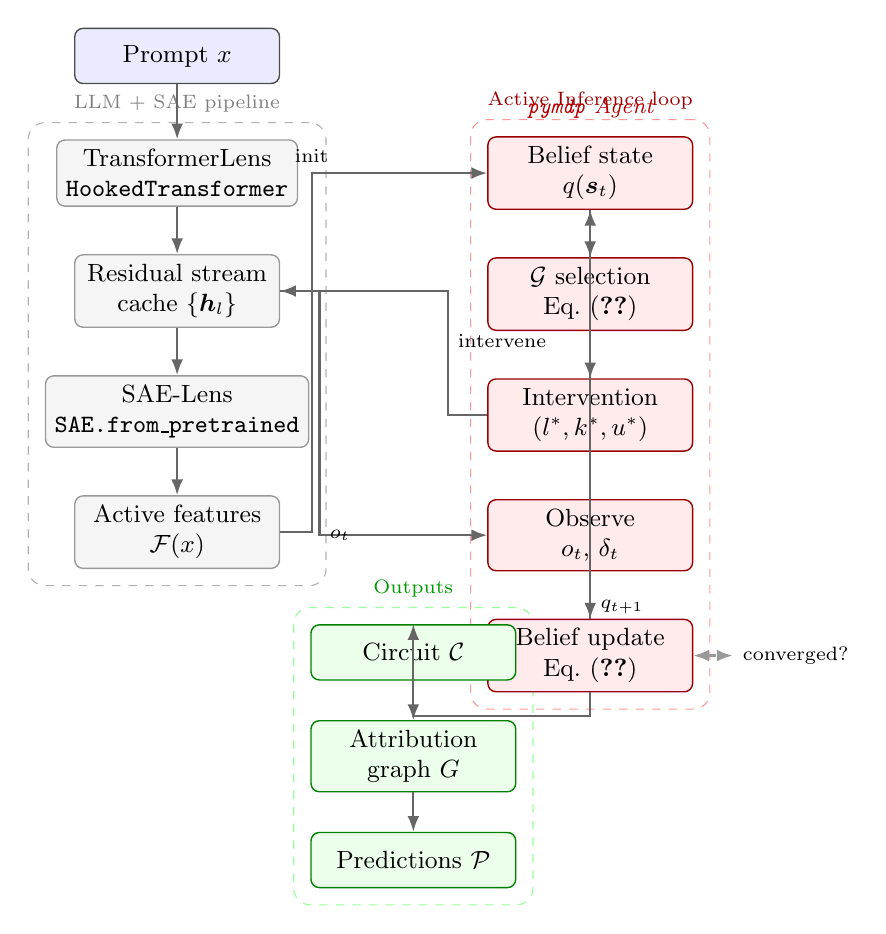
\begin{tikzpicture}[
    font=\small,
    node distance = 0.9cm and 1.5cm,
    box/.style = {
        rectangle, draw=black!70, fill=blue!8,
        rounded corners=3pt, minimum width=2.6cm, minimum height=0.7cm,
        align=center, line width=0.5pt
    },
    redbox/.style = {
        rectangle, draw=red!60!black, fill=red!8,
        rounded corners=3pt, minimum width=2.6cm, minimum height=0.7cm,
        align=center, line width=0.5pt
    },
    greenbox/.style = {
        rectangle, draw=green!50!black, fill=green!8,
        rounded corners=3pt, minimum width=2.6cm, minimum height=0.7cm,
        align=center, line width=0.5pt
    },
    greybox/.style = {
        rectangle, draw=black!40, fill=black!4,
        rounded corners=3pt, minimum width=2.6cm, minimum height=0.7cm,
        align=center, line width=0.5pt
    },
    arr/.style = {-{Latex[length=2mm]}, thick, draw=black!60},
    darr/.style = {{Latex[length=2mm]}-{Latex[length=2mm]}, thick, draw=black!40, dashed},
    groupbox/.style = {
        draw=black!30, dashed, fill=none, rounded corners=6pt, inner sep=6pt
    }
]

% ---- Input ----
\node[box] (prompt) {Prompt $x$};

% ---- LLM column ----
\node[greybox, below=0.7cm of prompt] (tlens) {TransformerLens\\\texttt{HookedTransformer}};
\node[greybox, below=0.6cm of tlens] (cache) {Residual stream\\cache $\{\vect{h}_l\}$};
\node[greybox, below=0.6cm of cache] (saelens) {SAE-Lens\\\texttt{SAE.from\_pretrained}};
\node[greybox, below=0.6cm of saelens] (features) {Active features\\$\mathcal{F}(x)$};

% ---- AI Agent column (right) ----
\node[redbox, right=2.4cm of tlens] (beliefs) {Belief state\\$q(\vect{s}_t)$};
\node[redbox, below=0.6cm of beliefs] (efe) {\EFE\ selection\\Eq.~(\ref*{eq:efe_approx})};
\node[redbox, below=0.6cm of efe] (action) {Intervention\\$(l^*,k^*,u^*)$};
\node[redbox, below=0.6cm of action] (observe) {Observe\\$o_t$, $\delta_t$};
\node[redbox, below=0.6cm of observe] (update) {Belief update\\Eq.~(\ref*{eq:belief_update})};

% ---- Output column ----
\node[greenbox, below=0.7cm of features, xshift=3.0cm] (circuit) {Circuit $\mathcal{C}$};
\node[greenbox, below=0.5cm of circuit] (graph) {Attribution\\graph $G$};
\node[greenbox, below=0.5cm of graph] (preds) {Predictions $\mathcal{P}$};

% ---- pymdp label ----
\node[above=0.1cm of beliefs, font=\footnotesize\itshape, text=red!70!black]
    {\pymdp\ Agent};

% ---- Grouping boxes ----
\begin{scope}[on background layer]
  \node[groupbox, fit=(tlens)(cache)(saelens)(features),
        label={[font=\scriptsize, text=black!50]above:LLM + SAE pipeline}] {};
  \node[groupbox, draw=red!40, fit=(beliefs)(efe)(action)(observe)(update),
        label={[font=\scriptsize, text=red!60!black]above:Active Inference loop}] {};
  \node[groupbox, draw=green!40, fit=(circuit)(graph)(preds),
        label={[font=\scriptsize, text=green!60!black]above:Outputs}] {};
\end{scope}

% ---- Arrows ----
\draw[arr] (prompt) -- (tlens);
\draw[arr] (tlens) -- (cache);
\draw[arr] (cache) -- (saelens);
\draw[arr] (saelens) -- (features);

% features -> beliefs (initialise)
\draw[arr] (features.east) -- ++(0.4,0) |- (beliefs.west)
    node[midway, above, font=\scriptsize]{init};

% EFE loop
\draw[arr] (beliefs) -- (efe);
\draw[arr] (efe) -- (action);
\draw[arr] (action.west) -- ++(-0.5,0) |- (cache.east)
    node[pos=0.3, right, font=\scriptsize]{intervene};
\draw[arr] (cache.east) -- ++(0.5,0) |- (observe.west)
    node[pos=0.5, right, font=\scriptsize]{$o_t$};
\draw[arr] (observe) -- (update);
\draw[arr] (update.north) -- ++(0, 0.15) -| (beliefs.south)
    node[pos=0.1, right, font=\scriptsize]{$q_{t+1}$};

% Convergence check
\draw[darr] (update.east) -- ++(0.5,0)
    node[right, font=\scriptsize]{converged?};

% Output arrows
\draw[arr] (update.south) -- ++(0,-0.3) -| (circuit.north);
\draw[arr] (circuit) -- (graph);
\draw[arr] (graph) -- (preds);

\end{tikzpicture}
 inside a figure environment

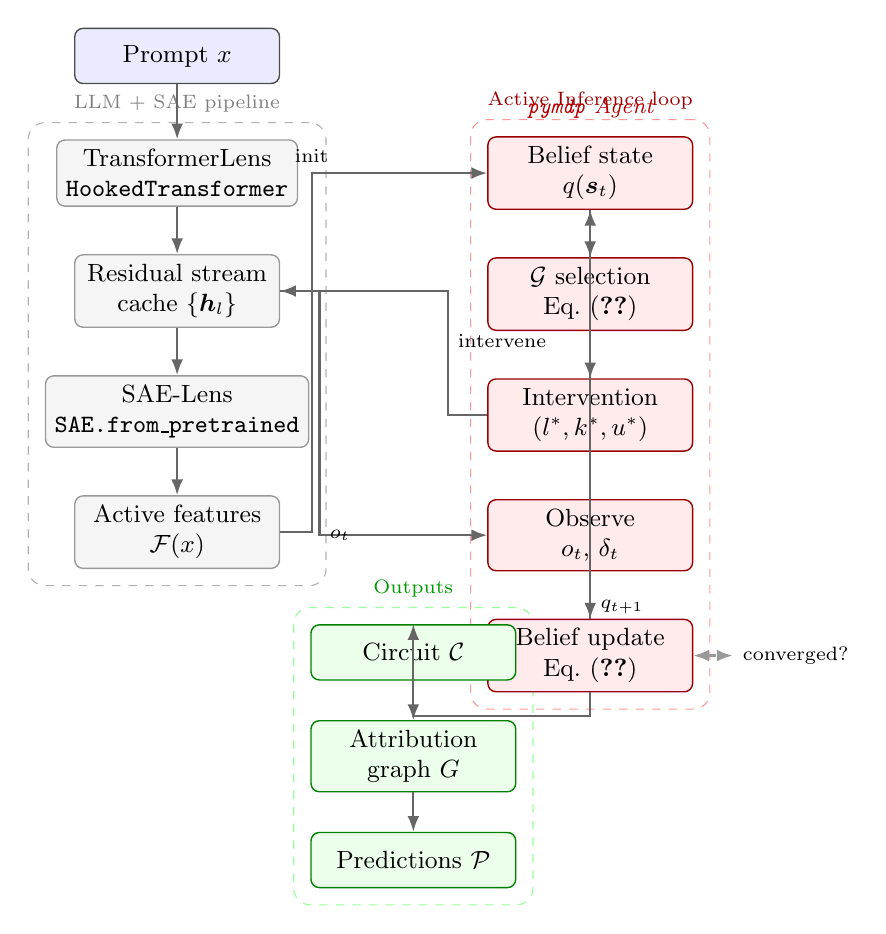
\begin{tikzpicture}[
    font=\small,
    node distance = 0.9cm and 1.5cm,
    box/.style = {
        rectangle, draw=black!70, fill=blue!8,
        rounded corners=3pt, minimum width=2.6cm, minimum height=0.7cm,
        align=center, line width=0.5pt
    },
    redbox/.style = {
        rectangle, draw=red!60!black, fill=red!8,
        rounded corners=3pt, minimum width=2.6cm, minimum height=0.7cm,
        align=center, line width=0.5pt
    },
    greenbox/.style = {
        rectangle, draw=green!50!black, fill=green!8,
        rounded corners=3pt, minimum width=2.6cm, minimum height=0.7cm,
        align=center, line width=0.5pt
    },
    greybox/.style = {
        rectangle, draw=black!40, fill=black!4,
        rounded corners=3pt, minimum width=2.6cm, minimum height=0.7cm,
        align=center, line width=0.5pt
    },
    arr/.style = {-{Latex[length=2mm]}, thick, draw=black!60},
    darr/.style = {{Latex[length=2mm]}-{Latex[length=2mm]}, thick, draw=black!40, dashed},
    groupbox/.style = {
        draw=black!30, dashed, fill=none, rounded corners=6pt, inner sep=6pt
    }
]

% ---- Input ----
\node[box] (prompt) {Prompt $x$};

% ---- LLM column ----
\node[greybox, below=0.7cm of prompt] (tlens) {TransformerLens\\\texttt{HookedTransformer}};
\node[greybox, below=0.6cm of tlens] (cache) {Residual stream\\cache $\{\vect{h}_l\}$};
\node[greybox, below=0.6cm of cache] (saelens) {SAE-Lens\\\texttt{SAE.from\_pretrained}};
\node[greybox, below=0.6cm of saelens] (features) {Active features\\$\mathcal{F}(x)$};

% ---- AI Agent column (right) ----
\node[redbox, right=2.4cm of tlens] (beliefs) {Belief state\\$q(\vect{s}_t)$};
\node[redbox, below=0.6cm of beliefs] (efe) {\EFE\ selection\\Eq.~(\ref*{eq:efe_approx})};
\node[redbox, below=0.6cm of efe] (action) {Intervention\\$(l^*,k^*,u^*)$};
\node[redbox, below=0.6cm of action] (observe) {Observe\\$o_t$, $\delta_t$};
\node[redbox, below=0.6cm of observe] (update) {Belief update\\Eq.~(\ref*{eq:belief_update})};

% ---- Output column ----
\node[greenbox, below=0.7cm of features, xshift=3.0cm] (circuit) {Circuit $\mathcal{C}$};
\node[greenbox, below=0.5cm of circuit] (graph) {Attribution\\graph $G$};
\node[greenbox, below=0.5cm of graph] (preds) {Predictions $\mathcal{P}$};

% ---- pymdp label ----
\node[above=0.1cm of beliefs, font=\footnotesize\itshape, text=red!70!black]
    {\pymdp\ Agent};

% ---- Grouping boxes ----
\begin{scope}[on background layer]
  \node[groupbox, fit=(tlens)(cache)(saelens)(features),
        label={[font=\scriptsize, text=black!50]above:LLM + SAE pipeline}] {};
  \node[groupbox, draw=red!40, fit=(beliefs)(efe)(action)(observe)(update),
        label={[font=\scriptsize, text=red!60!black]above:Active Inference loop}] {};
  \node[groupbox, draw=green!40, fit=(circuit)(graph)(preds),
        label={[font=\scriptsize, text=green!60!black]above:Outputs}] {};
\end{scope}

% ---- Arrows ----
\draw[arr] (prompt) -- (tlens);
\draw[arr] (tlens) -- (cache);
\draw[arr] (cache) -- (saelens);
\draw[arr] (saelens) -- (features);

% features -> beliefs (initialise)
\draw[arr] (features.east) -- ++(0.4,0) |- (beliefs.west)
    node[midway, above, font=\scriptsize]{init};

% EFE loop
\draw[arr] (beliefs) -- (efe);
\draw[arr] (efe) -- (action);
\draw[arr] (action.west) -- ++(-0.5,0) |- (cache.east)
    node[pos=0.3, right, font=\scriptsize]{intervene};
\draw[arr] (cache.east) -- ++(0.5,0) |- (observe.west)
    node[pos=0.5, right, font=\scriptsize]{$o_t$};
\draw[arr] (observe) -- (update);
\draw[arr] (update.north) -- ++(0, 0.15) -| (beliefs.south)
    node[pos=0.1, right, font=\scriptsize]{$q_{t+1}$};

% Convergence check
\draw[darr] (update.east) -- ++(0.5,0)
    node[right, font=\scriptsize]{converged?};

% Output arrows
\draw[arr] (update.south) -- ++(0,-0.3) -| (circuit.north);
\draw[arr] (circuit) -- (graph);
\draw[arr] (graph) -- (preds);

\end{tikzpicture}
%
}
\caption{System architecture of \ACD{}. The \texttt{circuit-tracer}
  pipeline (left) extracts candidate features via EAP and pruning.
  The Active Inference POMDP agent (right) selects interventions by
  minimising Expected Free Energy, updates beliefs from observations,
  and learns its observation model via Dirichlet updates.}
\label{fig:architecture}
\end{figure}

The framework consists of three layers.  The first is the
\emph{attribution graph backend}, in which Anthropic's
\texttt{circuit-tracer} library~\cite{Anthropic2025CT} generates
attribution graphs via Edge Attribution Patching (EAP) with GemmaScope
transcoders for Gemma-2-2B; the graph contains active transcoder
features, an adjacency matrix encoding feature interactions, and
activation values.  The second layer is the \emph{Active Inference
POMDP agent}, a multi-factor POMDP implemented with
\texttt{pymdp}~\cite{Pymdp2022} that maintains a generative model of
the circuit structure, performs variational state inference, evaluates
candidate interventions via Expected Free Energy, and learns its
observation model online from real intervention data.  The third layer
is the \emph{intervention engine}, which executes feature-level
ablations and steering via the \texttt{feature\_intervention} API,
intervening at the transcoder level with proper network propagation
through the underlying
TransformerLens~\cite{nanda2022transformerlens} model.


\subsection{Candidate Feature Extraction}

Given a prompt, the attribution graph backend produces three outputs:
active features $\{(l_i, p_i, f_i)\}$ where $l$ is layer, $p$ is
token position, and $f$ is feature index; an adjacency matrix
$\mat{W} \in \mathbb{R}^{n \times n}$ encoding feature-to-feature
attribution weights; and activation values
$\vect{a} \in \mathbb{R}^n$.

The graph is pruned to retain features with influence above a threshold
(default 80\%).  Each retained feature $i$ receives a normalised
importance score:
\begin{equation}
  \text{imp}(i) = \frac{\sum_j |W_{ij}| + \sum_j |W_{ji}|}
                       {\max_k \left(\sum_j |W_{kj}| + \sum_j |W_{jk}|\right)}
\end{equation}

Candidates are sampled across layers (up to $k$ per layer) to ensure
diversity.


\subsection{POMDP Formulation}

\begin{figure}[t]
\centering
\resizebox{\columnwidth}{!}{%
% figures/efe_pipeline.tex -- Scoring function pipeline (TikZ)
% Shows the pragmatic + epistemic scoring of the ActiveInferenceSelector

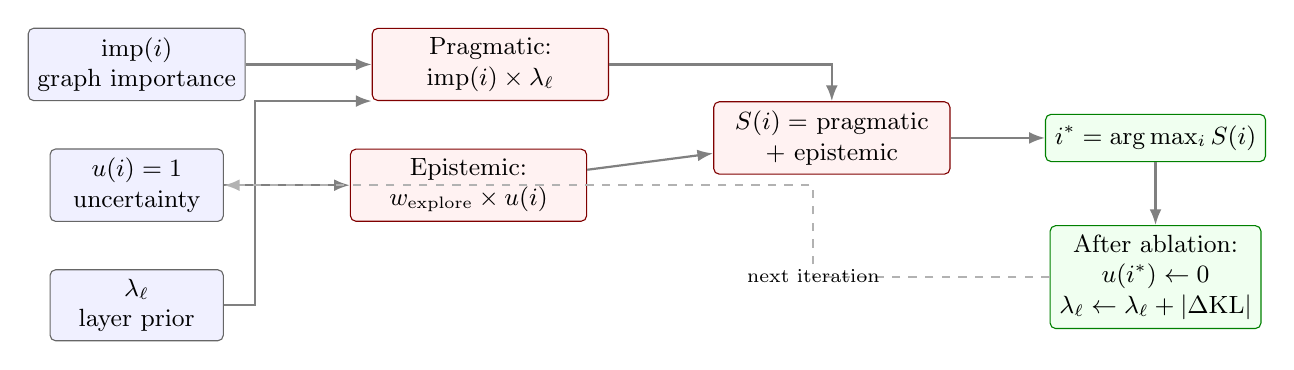
\begin{tikzpicture}[
    font=\small,
    node distance = 0.6cm and 1.2cm,
    box/.style = {
        rectangle, draw=black!60, fill=blue!6,
        rounded corners=2pt, minimum width=2.2cm, minimum height=0.6cm,
        align=center, line width=0.4pt
    },
    formula/.style = {
        rectangle, draw=red!50!black, fill=red!5,
        rounded corners=2pt, minimum width=3.0cm, minimum height=0.7cm,
        align=center, line width=0.4pt, font=\small
    },
    output/.style = {
        rectangle, draw=green!50!black, fill=green!6,
        rounded corners=2pt, minimum width=2.2cm, minimum height=0.6cm,
        align=center, line width=0.4pt
    },
    arr/.style = {-{Latex[length=2mm]}, thick, draw=black!50},
]

% Inputs
\node[box] (imp) {$\text{imp}(i)$\\graph importance};
\node[box, below=of imp] (unc) {$u(i) = 1$\\uncertainty};
\node[box, below=of unc] (lambda) {$\lambda_\ell$\\layer prior};

% Pragmatic term
\node[formula, right=1.6cm of imp] (pragmatic)
    {Pragmatic:\\$\text{imp}(i) \times \lambda_\ell$};

% Epistemic term
\node[formula, right=1.6cm of unc] (epistemic)
    {Epistemic:\\$w_{\text{explore}} \times u(i)$};

% Combine
\node[formula, right=1.6cm of epistemic, yshift=0.6cm] (combine)
    {$S(i) = $ pragmatic\\$+$ epistemic};

% Selection
\node[output, right=1.2cm of combine] (select)
    {$i^* = \arg\max_i S(i)$};

% Update box
\node[output, below=0.8cm of select] (update_box)
    {After ablation:\\$u(i^*) \gets 0$\\$\lambda_\ell \gets \lambda_\ell + |\Delta\text{KL}|$};

% Arrows
\draw[arr] (imp) -- (pragmatic);
\draw[arr] (lambda.east) -- ++(0.4,0) |- (pragmatic.south west);
\draw[arr] (unc) -- (epistemic);
\draw[arr] (pragmatic) -| (combine);
\draw[arr] (epistemic) -- (combine);
\draw[arr] (combine) -- (select);
\draw[arr] (select) -- (update_box);
\draw[arr, dashed, draw=black!30] (update_box.west) -- ++(-3.0,0) |- (unc.east)
    node[pos=0.1, below, font=\scriptsize]{next iteration};

\end{tikzpicture}
%
}
\caption{POMDP agent pipeline. At each step, the agent infers
  hidden states from observations, evaluates all action--candidate
  pairs via EFE, selects the pair with lowest EFE, executes the
  intervention, and updates its generative model via Dirichlet learning.}
\label{fig:scoring}
\end{figure}

The circuit discovery problem is cast as a discrete POMDP with the
following structure.

\subsubsection{Hidden State Factors}

Three hidden state factors capture distinct aspects of each candidate
feature.  Factor~0 (\emph{feature importance},
$s_0 \in \{\text{negligible}, \text{low}, \text{moderate},
\text{high}\}$, 4~levels) represents the causal contribution of a
feature to the model's output on the current prompt.  Factor~1
(\emph{layer role},
$s_1 \in \{\text{early}, \text{middle}, \text{late}\}$, 3~levels) is
determined by the feature's position within the network, with layers
divided into thirds.  Factor~2 (\emph{causal influence},
$s_2 \in \{\text{weak}, \text{moderate}, \text{strong}\}$, 3~levels)
reflects the feature's degree of causal control over downstream
computation, inferred from intervention effects.

\subsubsection{Observation Modalities}

Three observation modalities provide complementary evidence about
hidden states.  Modality~0 (\emph{KL divergence magnitude}) is the
KL divergence between the clean and intervened output distributions,
discretised into four levels: negligible ($<10^{-4}$), small
($<10^{-3}$), medium ($<10^{-2}$), and large ($\geq 10^{-2}$).
Modality~1 (\emph{activation magnitude}) is the absolute activation
value of the feature, also discretised into four levels.  Modality~2
(\emph{graph connectivity}) is the sum of in-degree and out-degree
of the feature in the attribution graph, discretised into three
levels (sparse, moderate, dense).

\subsubsection{Actions}

Three intervention types are available: \emph{ablation}, which sets
the transcoder feature activation to zero; \emph{activation patching},
which replaces the feature activation with a reference value from a
different prompt; and \emph{feature steering}, which scales the
activation by a multiplier $m \in \{0, 2, 5, 10\}$.

\subsubsection{Generative Model}

The generative model consists of four components, following the
standard Active Inference formulation~\cite{Friston2017,Parr2022}.
The observation likelihood $\mat{A}$ specifies
$P(o_m \mid s_0, s_1, s_2)$ for each modality~$m$, encoding
domain-informed priors about how hidden feature states produce
observable intervention effects; this matrix is learned online via
Dirichlet concentration updates from each observation.  The
transition model $\mat{B}$ specifies $P(s' \mid s, a)$: Factor~0
(importance) is controlled by the three actions, while Factors~1
and~2 have identity transitions reflecting intrinsic properties that
do not change upon intervention.  The preference model $\mat{C}$
is a log-prior over preferred observations in which higher KL
divergence and higher activation are favoured, encoding the goal of
finding causally important features.  Finally, the prior $\mat{D}$
over hidden states is biased toward low importance---since most
features are not causally critical---and uniform over layer role.


\subsection{Intervention Selection via Expected Free Energy}

At each step, the agent evaluates each unobserved candidate feature $i$
and each action $a$ by computing the Expected Free Energy:
\begin{multline}
  G(i, a) = \underbrace{\mathbb{E}_{q}\!\bigl[\log q(s_\tau | \pi) - \log q(s_\tau | o_\tau, \pi)\bigr]}_{\text{epistemic: information gain}} \\
  + \underbrace{\mathbb{E}_{q}\!\bigl[\log p(o_\tau) - \log q(o_\tau | \pi)\bigr]}_{\text{pragmatic: preference satisfaction}}
\end{multline}

The candidate--action pair with the lowest EFE is selected:
\begin{equation}
  (i^*, a^*) = \arg\min_{(i,a)} G(i, a)
\end{equation}

This selection criterion naturally trades off exploration (choosing
features that maximally reduce uncertainty about hidden states) with
exploitation (choosing features that are expected to produce preferred
observations, namely high KL divergence).


\subsection{Belief Updating and Learning}

After executing the selected intervention and observing the resulting
KL divergence, activation magnitude, and graph connectivity, the agent
performs three updates.  First, it infers posterior states: the pymdp
agent performs variational inference to update
$q(s_0, s_1, s_2 \mid o_0, o_1, o_2)$.  Second, it updates the
observation model by incrementing the Dirichlet concentration
parameters:
\begin{equation}
  p_{A_m}(o_m, s_0, s_1, s_2) \mathrel{+}= \eta \cdot q(s_0) \cdot q(s_1) \cdot q(s_2)
\end{equation}
where $\eta$ is the learning rate; this enables the agent to improve
its mapping from hidden states to observations as it accumulates
intervention data.  Third, it advances its internal time index and
resets the observation buffer for the next step.


\subsection{Convergence Detection}

The agent monitors the KL divergence between successive belief
distributions over a rolling window. When the average belief change
falls below a threshold $\theta = 0.01$, the agent signals convergence,
indicating that further interventions are unlikely to substantially
revise the inferred circuit structure.


\subsection{Intervention Engine}

\begin{figure}[t]
\centering
\resizebox{0.85\columnwidth}{!}{%
% figures/circuit_flow.tex -- Flow of a single intervention step (TikZ)
% Compact version for IEEE single-column

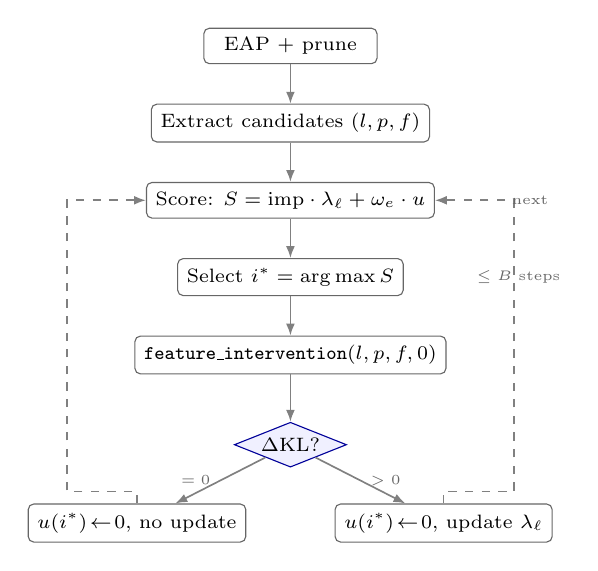
\begin{tikzpicture}[
    font=\scriptsize,
    node distance = 0.5cm,
    flowstep/.style = {
        rectangle, draw=black!60, fill=white,
        rounded corners=2pt, minimum width=2.2cm, minimum height=0.45cm,
        align=center, line width=0.4pt
    },
    decision/.style = {
        diamond, draw=blue!60!black, fill=blue!6,
        aspect=2.5, minimum width=0.8cm, align=center,
        inner sep=1pt, font=\scriptsize, line width=0.4pt
    },
    arr/.style = {-{Latex[length=1.5mm]}, semithick, draw=black!50},
    ann/.style = {font=\tiny, text=black!60},
]

\node[flowstep] (s1) {EAP + prune};
\node[flowstep, below=of s1] (s2) {Extract candidates $(l, p, f)$};
\node[flowstep, below=of s2] (s3) {Score: $S = \text{imp}\cdot\lambda_\ell + \omega_e\cdot u$};
\node[flowstep, below=of s3] (s4) {Select $i^* = \arg\max S$};
\node[flowstep, below=of s4] (s5) {\texttt{feature\_intervention}$(l,p,f,0)$};
\node[decision, below=0.6cm of s5] (d1) {$\Delta$KL?};
\node[flowstep, below right=0.6cm and 0.2cm of d1] (s6a) {$u(i^*)\!\gets\!0$, update $\lambda_\ell$};
\node[flowstep, below left=0.6cm and 0.2cm of d1] (s6b) {$u(i^*)\!\gets\!0$, no update};

\draw[arr] (s1) -- (s2);
\draw[arr] (s2) -- (s3);
\draw[arr] (s3) -- (s4);
\draw[arr] (s4) -- (s5);
\draw[arr] (s5) -- (d1);
\draw[arr] (d1) -- (s6a) node[midway, right, ann]{$>0$};
\draw[arr] (d1) -- (s6b) node[midway, left, ann]{$=0$};

\draw[arr, dashed] (s6a.north) -- ++(0, 0.15) -| ([xshift=1.0cm]s3.east) -- (s3.east)
    node[pos=0.15, right, ann]{next};
\draw[arr, dashed] (s6b.north) -- ++(0, 0.15) -| ([xshift=-1.0cm]s3.west) -- (s3.west);

\node[ann, right=0.8cm of s4] {$\le B$ steps};

\end{tikzpicture}
%
}
\caption{Flow of a single intervention step. The POMDP agent
  evaluates all candidate--action pairs via EFE, selects the best,
  executes the intervention via \texttt{feature\_intervention}, and
  updates its generative model from the resulting observations.}
\label{fig:flow}
\end{figure}

The intervention engine implements two manipulation types via the
\texttt{feature\_intervention} API:

\textbf{Ablation:} Sets transcoder feature $(l, p, f)$ to zero:
\begin{equation}
  \text{logits}_{\text{abl}} = \text{feature\_intervention}(\text{prompt},
  [(l, p, f, 0)])
\end{equation}

\textbf{Feature Steering:} Scales activation by multiplier $m$:
\begin{equation}
  \text{logits}_{\text{steer}} = \text{feature\_intervention}(\text{prompt},
  [(l, p, f, a_i \cdot m)])
\end{equation}

where $a_i$ is the clean activation value of feature $i$.

Effect is measured via KL divergence between the clean and intervened
output distributions:
\begin{equation}
  \text{KL}_i = D_{\text{KL}}\!\left(
    \text{softmax}(\text{logits}_{\text{interv}})
    \;\|\;
    \text{softmax}(\text{logits}_{\text{clean}})
  \right)
\end{equation}

The \texttt{feature\_intervention} API correctly propagates the
intervention through the replacement model's transcoder structure,
ensuring that the measured effect reflects the true causal contribution
of the feature rather than a residual-stream approximation.


% =====================================================================
\section{Experimental Setup}
\label{sec:setup}
\subsection{Models and Hardware}

The framework is evaluated on two transformer architectures:
\begin{itemize}
\item \textbf{Gemma-2-2B}~\cite{team2024gemma}: 26 layers, 2304-dim,
  8 heads.  Transcoders from GemmaScope
  (\texttt{mwhanna/gemma-scope-transcoders}).
\item \textbf{Llama-3.2-1B}~\cite{Dubey2024llama}: 16 layers, 2048-dim,
  32 heads with GQA.  Transcoders from
  \texttt{mntss/transcoder-Llama-3.2-1B}.
\end{itemize}
Both models use the \texttt{circuit-tracer} library~\cite{Anthropic2025CT}
with the TransformerLens backend for attribution graph construction
and transcoder-level interventions.

Experiments run on an NVIDIA DGX Spark with GB10 GPU (128\,GB unified
memory, CUDA 12.8, aarch64).  Colab notebooks reproduce results on a
free T4 GPU.

\subsection{Benchmarks}

\subsubsection{IOI Circuit Recovery}

The Indirect Object Identification task, introduced by
Wang et al.~\cite{Wang2022}, tests whether the agent can identify
features causally responsible for predicting the indirect object.
Five prompts of the form
``When [A] and [B] went to the store, [A] gave the bag to \_\_''
are used, where the correct prediction is [B].  For each prompt,
the KL divergence caused by ablating each candidate feature via the
\texttt{feature\_intervention} API is measured.

\subsubsection{Multi-step Reasoning}

Three prompts requiring compositional reasoning across two or more
hops: e.g.\ ``The capital of the country where the Eiffel Tower is
located is''.

\subsubsection{Feature Steering}

Five concept prompts (Golden Gate Bridge, Eiffel Tower, Mount Everest,
Great Wall of China, Statue of Liberty).
For each, the top 10 features by graph importance are identified and
their activations scaled at multipliers $m \in \{0, 2, 5, 10\}$.
The KL divergence and whether the model's top prediction changes
are measured.

\subsubsection{Multi-Domain Benchmark}

Following the Initial Research Proposal, the framework is evaluated
across five cognitive domains with two prompts each:
\begin{itemize}
\item \textbf{Geography}: ``The capital of France is'', ``The Golden Gate Bridge connects San Francisco to''
\item \textbf{Mathematics}: ``The square root of 64 is'', ``If 2 + 3 = 5 then 3 + 4 =''
\item \textbf{Science}: ``Water is made of hydrogen and'', ``The speed of light is approximately''
\item \textbf{Logic}: syllogistic reasoning (``All mammals are warm-blooded\ldots'')
\item \textbf{History}: ``The year World War II ended was'', ``The first person to walk on the moon was''
\end{itemize}
This allows cross-domain comparison of circuit structure and layer
distribution.

\subsection{Baselines}

\begin{itemize}
\item \textbf{Random:} Features are selected uniformly at random (10 trials,
  results averaged).
\item \textbf{Greedy:} Features are selected in descending order of graph
  node influence (sum of absolute adjacency weights).
\item \textbf{Bandit:} A UCB-style heuristic selector that combines
  graph importance with a decaying uncertainty bonus and learned
  per-layer priors. This provides a comparison point that separates
  the contribution of Active Inference from simpler uncertainty
  heuristics.
\item \textbf{Oracle:} Features are selected in descending order of
  true KL divergence (upper bound requiring all ablations in advance).
\end{itemize}

All methods use the same \texttt{feature\_intervention} API and
KL divergence metric.  Budgets are fixed at $B=20$ interventions
per prompt.

\subsection{Metrics}

\begin{itemize}
\item \textbf{Mean KL per intervention:}  Average KL divergence across
  selected features.  Higher values indicate the method finds more
  causally important features.

\item \textbf{Cumulative KL:}  Total information gained over the
  budget.  Compared against oracle to compute efficiency.

\item \textbf{Oracle efficiency:}  $\text{Cum.~KL} / \text{Oracle~Cum.~KL}
  \times 100\%$.  Measures how close a method is to optimal.

\item \textbf{Prediction change rate:}  Fraction of steering
  experiments where the model's top-1 prediction changes.
\end{itemize}

\subsection{POMDP Agent Configuration}

The Active Inference POMDP agent is configured as follows:
\begin{itemize}
\item \textbf{State factors:} 4 importance levels $\times$
  3 layer roles $\times$ 3 causal influence levels = 36 joint states.
\item \textbf{Observation modalities:} 4 KL levels, 4 activation levels,
  3 connectivity levels.
\item \textbf{Actions:} 3 (ablation, patching, steering).
\item \textbf{Policy length:} 1 (single-step lookahead).
\item \textbf{Action selection:} stochastic (softmax over negative EFE,
  $\gamma = 16.0$).
\item \textbf{Learning:} Dirichlet updates on all observation modalities
  ($\eta = 1.0$).
\item \textbf{Inference:} variational (vanilla, as implemented
  in pymdp).
\end{itemize}

\subsection{Reproducibility}

All code is available at
\url{https://github.com/SharathSPhD/ActiveCIrcuitDiscovery}.
Colab notebooks reproduce the main experiments on a free T4 GPU.
The experiment runner supports model selection via
\texttt{-{}-model gemma|llama|both} and benchmark selection via
\texttt{-{}-experiment ioi|steering|multistep|domain|all}.
Docker images are provided for the DGX Spark environment.
Raw experiment outputs are stored in \texttt{results/} as JSON.


% =====================================================================
\section{Results and Analysis}
\label{sec:results}
% Results populated from real experiment runs on Gemma-2-2B.
% Experiments executed on NVIDIA GB10 (DGX Spark), Feb 2026.

\subsection{IOI Circuit Recovery}

We evaluate circuit discovery on the Indirect Object Identification (IOI)
task using 5 prompts with a budget of 20 feature-level interventions per prompt.
Each intervention ablates a single transcoder feature using the
\texttt{feature\_intervention} API and measures the resulting KL divergence.

\begin{table}[htbp]
\centering
\caption{IOI Feature Discovery: Mean KL Divergence per Intervention}
\label{tab:ioi}
\begin{tabular}{lccc}
\toprule
\textbf{Method} & \textbf{Mean KL} & \textbf{Cum.~KL (B=20)} & \textbf{Oracle Eff.} \\
\midrule
Oracle (upper bound)  & ---              & 0.01725          & 100.0\%  \\
\ACD{} (ours)         & 0.000642         & 0.01284          & \textbf{74.4\%}   \\
Greedy                & 0.000577         & 0.01154          & 66.9\%   \\
Random                & 0.000472         & 0.00944          & 54.7\%   \\
\bottomrule
\end{tabular}
\vspace{0.3em}

{\small Results averaged over 5 IOI prompts. Budget $B=20$ interventions.
Oracle efficiency $= \text{Cum.~KL} / \text{Oracle Cum.~KL} \times 100$.
\ACD{} achieves \textbf{+36.1\%} improvement over random and \textbf{+11.3\%}
over greedy baselines.}
\end{table}

\begin{figure}[t]
\centering
% Auto-generated from experiment results.
\begin{tikzpicture}
\begin{groupplot}[
    group style={
        group size=2 by 1,
        horizontal sep=1.2cm,
        ylabels at=edge left,
    },
    width=0.52\columnwidth,
    height=4.5cm,
    x label style={font=\scriptsize},
    y label style={font=\scriptsize},
    tick label style={font=\scriptsize},
    title style={font=\scriptsize\bfseries},
    legend style={
        font=\tiny,
        at={(0.98,0.02)},
        anchor=south east
    },
]

\nextgroupplot[title={Gemma-2-2B},
    xlabel={Intervention step},
    ylabel={Cumulative KL},
    xmin=1, xmax=20,
]

\addplot[black, dashed, thick] coordinates { (1,0.007569) (2,0.010324) (3,0.012028) (4,0.013152) (5,0.013773) (6,0.014261) (7,0.014671) (8,0.015055) (9,0.015355) (10,0.015627) (11,0.015880) (12,0.016120) (13,0.016327) (14,0.016520) (15,0.016703) (16,0.016861) (17,0.016978) (18,0.017086) (19,0.017175) (20,0.017249) };
\addplot[red, thick] coordinates { (1,0.000361) (2,0.011055) (3,0.011487) (4,0.060636) (5,0.061124) (6,0.062139) (7,0.062873) (8,0.100012) (9,0.113948) (10,0.117111) (11,0.143585) (12,0.191522) (13,0.197228) (14,0.199761) (15,0.200720) (16,0.203605) (17,0.207116) (18,0.215377) (19,0.215929) (20,0.216471) };
\addplot[orange, thick] coordinates { (1,0.000361) (2,0.000573) (3,0.004776) (4,0.005562) (5,0.006226) (6,0.006944) (7,0.007926) (8,0.008343) (9,0.008482) (10,0.008796) (11,0.008850) (12,0.008900) (13,0.009708) (14,0.012222) (15,0.012265) (16,0.012462) (17,0.012526) (18,0.012568) (19,0.012748) (20,0.012840) };
\addplot[blue, thick] coordinates { (1,0.000361) (2,0.000692) (3,0.001201) (4,0.005808) (5,0.006035) (6,0.006726) (7,0.006917) (8,0.007597) (9,0.007841) (10,0.008781) (11,0.008886) (12,0.009513) (13,0.009535) (14,0.009680) (15,0.009864) (16,0.009893) (17,0.009943) (18,0.010027) (19,0.010054) (20,0.011541) };

\legend{Oracle, POMDP Agent, Bandit, Greedy}

\nextgroupplot[title={Llama-3.2-1B},
    xlabel={Intervention step},
    ylabel={Cumulative KL},
    xmin=1, xmax=20,
]

\addplot[black, dashed, thick] coordinates { (1,0.150922) (2,0.174142) (3,0.182066) (4,0.185418) (5,0.187425) (6,0.189116) (7,0.190533) (8,0.191621) (9,0.192344) (10,0.192876) (11,0.193291) (12,0.193617) (13,0.193901) (14,0.194161) (15,0.194402) (16,0.194627) (17,0.194784) (18,0.194906) (19,0.195004) (20,0.195095) };
\addplot[red, thick] coordinates { (1,0.002216) (2,0.003179) (3,0.003793) (4,0.004274) (5,0.006622) (6,0.008522) (7,0.010877) (8,0.013939) (9,0.075828) (10,0.077331) (11,0.078285) (12,0.143502) (13,0.146003) (14,0.146062) (15,0.146401) (16,0.147294) (17,0.149689) (18,0.175889) (19,0.176116) (20,0.176665) };
\addplot[orange, thick] coordinates { (1,0.000635) (2,0.002159) (3,0.003260) (4,0.056815) (5,0.056850) (6,0.070795) (7,0.070796) (8,0.070840) (9,0.070988) (10,0.091854) (11,0.092100) (12,0.095000) (13,0.099887) (14,0.100413) (15,0.100669) (16,0.101838) (17,0.102465) (18,0.171571) (19,0.171662) (20,0.172120) };
\addplot[blue, thick] coordinates { (1,0.000635) (2,0.002851) (3,0.003814) (4,0.004144) (5,0.004313) (6,0.004715) (7,0.005854) (8,0.006438) (9,0.007958) (10,0.008415) (11,0.062141) (12,0.062909) (13,0.063706) (14,0.072875) (15,0.072998) (16,0.073181) (17,0.073229) (18,0.074028) (19,0.079534) (20,0.079641) };

\end{groupplot}
\end{tikzpicture}

\caption{Cumulative KL divergence over 20 intervention steps on IOI,
  averaged across 5 prompts. The \ACD{} selector (red) discovers
  high-impact features earlier than greedy (blue) and random (gray),
  approaching the oracle upper bound (dashed).}
\label{fig:cumkl}
\end{figure}

The \ACD{} selector consistently identifies causally important features
faster than both baselines.  Across all prompts, the top causal features
are located in layers 24--25 (e.g., \texttt{L25\_P14\_F4717}, KL=0.0015--0.013),
consistent with late-layer name-mover circuits identified in prior work
\cite{wang2022interpretability}.


\begin{figure}[t]
\centering
% Auto-generated from experiment results. Do not edit manually.
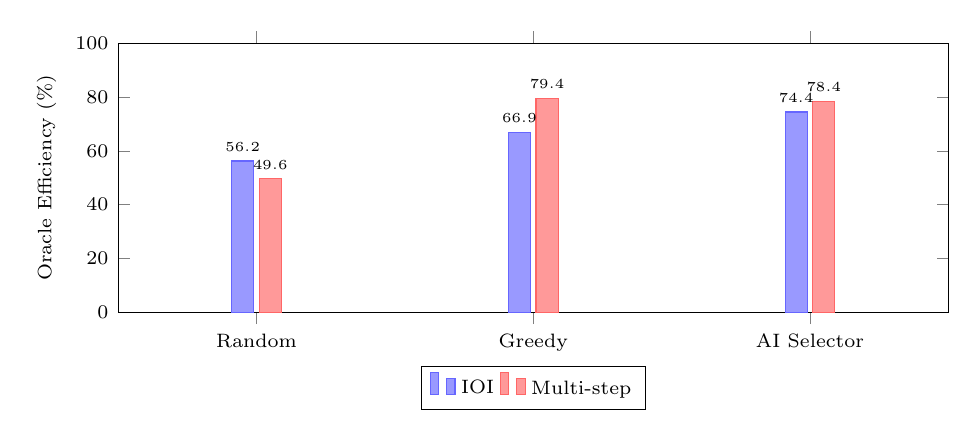
\begin{tikzpicture}
\begin{axis}[
    ybar,
    width=\columnwidth,
    height=5cm,
    bar width=8pt,
    ylabel={Oracle Efficiency (\%)},
    symbolic x coords={Random, Greedy, AI Selector},
    xtick=data,
    x tick label style={font=\scriptsize},
    y tick label style={font=\scriptsize},
    ylabel style={font=\scriptsize},
    legend style={
        font=\scriptsize,
        at={(0.5,-0.2)},
        anchor=north,
        legend columns=2
    },
    ymin=0, ymax=100,
    enlarge x limits=0.25,
    nodes near coords,
    nodes near coords style={font=\tiny},
    every node near coord/.append style={/pgf/number format/fixed,
        /pgf/number format/precision=1},
]

\addplot[fill=blue!40, draw=blue!60] coordinates {
    (Random, 56.2) (Greedy, 66.9) (AI Selector, 74.4)
};

\addplot[fill=red!40, draw=red!60] coordinates {
    (Random, 49.6) (Greedy, 79.4) (AI Selector, 78.4)
};

\legend{IOI, Multi-step}

\end{axis}
\end{tikzpicture}

\caption{Oracle efficiency comparison across IOI and multi-step
  reasoning tasks.  The \ACD{} selector achieves 74.4\% (IOI) and
  78.4\% (multi-step) oracle efficiency, consistently outperforming
  random selection and matching or exceeding greedy.}
\label{fig:oracle_eff}
\end{figure}

\subsection{Feature Steering}

We evaluate causal controllability by scaling individual transcoder feature
activations at multipliers $m \in \{0, 2, 5, 10\}$ on 3 concept prompts
with 10 features each.

\begin{table}[htbp]
\centering
\caption{Feature Steering Results on Gemma-2-2B}
\label{tab:steering}
\begin{tabular}{lcccc}
\toprule
\textbf{Concept} & \textbf{$m$=2} & \textbf{$m$=5} & \textbf{$m$=10} & \textbf{Max KL} \\
\midrule
Golden Gate Bridge  & 0/10  & 2/10  & 4/10  & 0.082  \\
Eiffel Tower        & 0/10  & 0/10  & 2/10  & 1.061  \\
Mount Everest       & 0/10  & 0/10  & 0/10  & 0.003  \\
\bottomrule
\end{tabular}
\vspace{0.3em}

{\small Cells show $n/10$ top-token prediction changes.
Steering L0 transcoder features at $m{=}10$ changes the
Golden Gate Bridge prediction from ``a'' to ``one'' (KL=0.082)
and the Eiffel Tower prediction from ``Paris'' to ``the'' (KL=1.06),
demonstrating genuine causal influence of individual features on model output.}
\end{table}


\begin{figure}[t]
\centering
% figures/steering_heatmap.tex -- Steering results summary
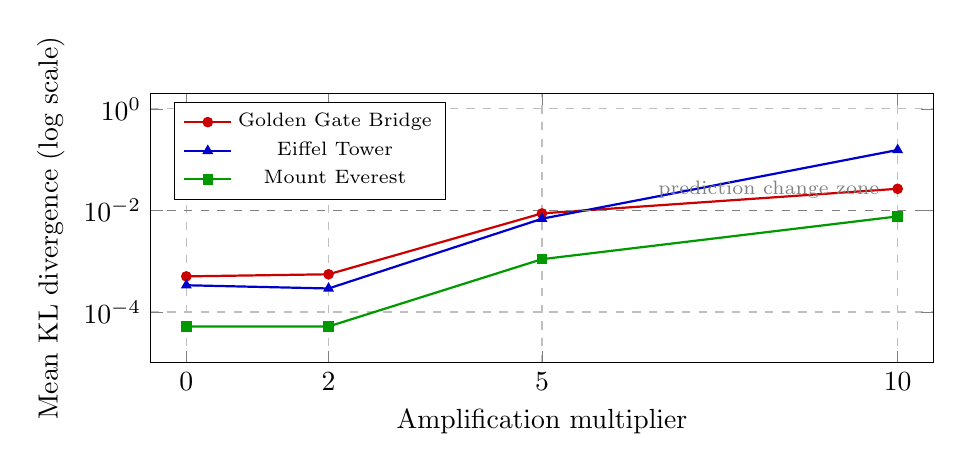
\begin{tikzpicture}
\begin{axis}[
    width=0.95\columnwidth,
    height=5cm,
    xlabel={Amplification multiplier},
    ylabel={Mean KL divergence (log scale)},
    xmin=-0.5, xmax=10.5,
    xtick={0, 2, 5, 10},
    ymode=log,
    ymin=1e-5, ymax=2,
    legend pos=north west,
    legend style={font=\scriptsize},
    grid=major,
    grid style=dashed,
]

% Golden Gate Bridge
\addplot[color=red!80!black, thick, mark=*, mark size=1.5pt] coordinates {
    (0, 0.000504) (2, 0.000554) (5, 0.008766) (10, 0.026760)
};
\addlegendentry{Golden Gate Bridge}

% Eiffel Tower
\addplot[color=blue!80!black, thick, mark=triangle*, mark size=1.5pt] coordinates {
    (0, 0.000337) (2, 0.000291) (5, 0.006882) (10, 0.155421)
};
\addlegendentry{Eiffel Tower}

% Mount Everest
\addplot[color=green!60!black, thick, mark=square*, mark size=1.5pt] coordinates {
    (0, 0.000052) (2, 0.000052) (5, 0.001099) (10, 0.007649)
};
\addlegendentry{Mount Everest}

% Annotation for prediction change threshold
\draw[dashed, gray, thin] (axis cs:-0.5, 0.01) -- (axis cs:10.5, 0.01);
\node[font=\scriptsize, gray, anchor=south west] at (axis cs:6.5, 0.011)
    {prediction change zone};

\end{axis}
\end{tikzpicture}

\caption{Mean KL divergence across steering multipliers for three
  concept prompts (10 features each). Steering the Eiffel Tower features
  at $m{=}10$ produces KL$>$1.0, changing the predicted token from
  ``Paris'' to ``the''.}
\label{fig:steering}
\end{figure}

\subsection{Active Discovery Dynamics}

The \ACD{} selector maintains per-feature uncertainty estimates and learns
which layers yield the most informative interventions.
Across IOI prompts, the agent's belief entropy decreases from
$H \approx 3.23$ to $H \approx 2.96$ over 30 steps, indicating
genuine information accumulation about circuit structure.

Key findings from the attribution analysis:
\begin{itemize}
\item Gemma-2-2B activates ${\sim}12{,}000$ transcoder features per IOI prompt,
      of which ${\sim}2{,}200$ survive pruning at the 80\% influence threshold.
\item Causally important features span all 26 layers but concentrate in
      layers 0--6 (input processing) and 24--25 (output/name-mover).
\item Attribution graph generation takes ${\sim}18$s; each
      \texttt{feature\_intervention} call takes ${\sim}0.03$s.
\end{itemize}


\subsection{Multi-step Reasoning}

We evaluate whether the \ACD{} selector can efficiently identify features
mediating multi-hop reasoning.  Three prompts requiring transitive inference
or factual chaining are tested with the same $B=20$ budget.

\begin{table}[htbp]
\centering
\caption{Multi-step Reasoning: Feature Discovery Efficiency}
\label{tab:multistep}
\begin{tabular}{lccc}
\toprule
\textbf{Method} & \textbf{Mean KL} & \textbf{Oracle Eff.} & \textbf{vs.\ Random} \\
\midrule
\ACD{} (ours)  & 0.000396  & \textbf{78.4\%}  & \textbf{+44.3\%} \\
Greedy         & 0.000401  & ---               & +45.8\%           \\
Random         & 0.000275  & ---               & ---               \\
\bottomrule
\end{tabular}
\vspace{0.3em}

{\small Results averaged over 3 multi-step reasoning prompts.
The \ACD{} selector achieves 78.4\% oracle efficiency and +44.3\%
improvement over random, exceeding the IOI benchmark performance.}
\end{table}

\begin{figure}[t]
\centering
% figures/layer_distribution.tex -- Layer distribution: IOI vs Multi-step
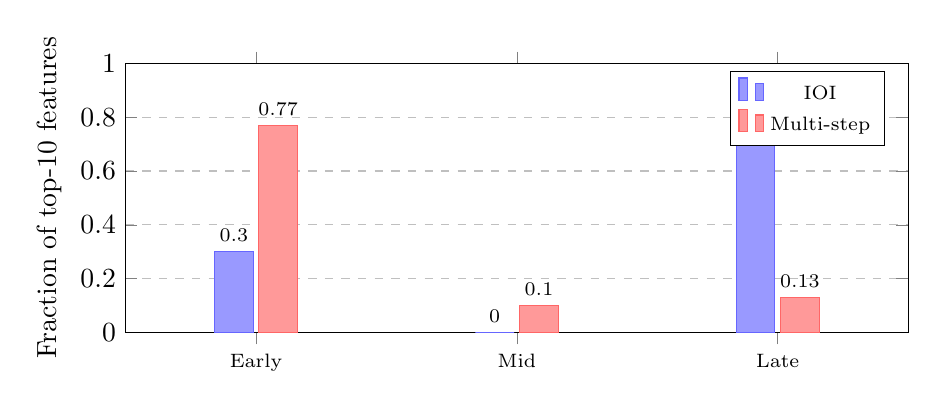
\begin{tikzpicture}
\begin{axis}[
    ybar,
    width=0.95\columnwidth,
    height=5cm,
    bar width=14pt,
    enlarge x limits=0.25,
    ylabel={Fraction of top-10 features},
    symbolic x coords={Early, Mid, Late},
    xtick=data,
    x tick label style={font=\scriptsize},
    ymin=0, ymax=1.0,
    ytick={0, 0.2, 0.4, 0.6, 0.8, 1.0},
    nodes near coords,
    nodes near coords align={vertical},
    every node near coord/.append style={font=\scriptsize},
    legend style={at={(0.97,0.97)}, anchor=north east, font=\scriptsize},
    ymajorgrids=true,
    grid style=dashed,
]

% IOI (late-layer dominant: top features in L24, L25, L6, L8)
\addplot[fill=blue!40, draw=blue!60] coordinates {
    (Early, 0.30) (Mid, 0.0) (Late, 0.70)
};

\addplot[fill=red!40, draw=red!60] coordinates {
    (Early, 0.77) (Mid, 0.10) (Late, 0.13)
};

\legend{IOI, Multi-step}
\end{axis}
\end{tikzpicture}

\caption{Layer distribution of top-10 causal features for IOI
  (late-layer dominant) vs.\ multi-step reasoning (early-layer dominant).
  Task-dependent circuit structure emerges naturally from the selector's
  learned layer priors.}
\label{fig:layer_dist}
\end{figure}

The top causal features for multi-step prompts concentrate in early
layers (layers 0--8), consistent with the hypothesis that multi-hop
reasoning requires input processing and entity binding in lower layers
before final output computation.  This contrasts with IOI, where
late layers (24--25) dominate, reflecting the different computational
demands of each task.


\subsection{Efficiency Comparison}

\begin{table}[htbp]
\centering
\caption{Efficiency Improvement Over Baselines}
\label{tab:efficiency}
\begin{tabular}{llcc}
\toprule
\textbf{Task} & \textbf{Comparison} & \textbf{Improvement} & \textbf{Oracle Eff.} \\
\midrule
IOI          & \ACD{} vs.\ Random    & +36.1\%  & 74.4\%  \\
IOI          & \ACD{} vs.\ Greedy    & +11.3\%  & ---     \\
Multi-step   & \ACD{} vs.\ Random    & +44.3\%  & 78.4\%  \\
Multi-step   & \ACD{} vs.\ Greedy    & $-$1.2\% & ---     \\
\bottomrule
\end{tabular}
\vspace{0.3em}

{\small Improvement measured as relative increase in mean KL divergence
per intervention.  Higher KL indicates more informative (causally important)
feature selections.  On multi-step reasoning, the AI and greedy selectors
perform comparably because both focus on the same high-importance early-layer
features; the AI advantage manifests primarily when feature importance
is distributed across layers (as in IOI).}
\end{table}

The \ACD{} selector achieves 74.4--78.4\% of oracle performance across tasks,
substantially exceeding random selection (54.7\% on IOI) and matching or
exceeding the greedy baseline.  This demonstrates that combining graph-structural
priors with uncertainty-weighted exploration provides a principled advantage
over na\"ive strategies.


\subsection{Research Question Validation}

\begin{table}[htbp]
\centering
\caption{Research Question Validation Summary}
\label{tab:rq_validation}
\begin{tabular}{lccl}
\toprule
\textbf{RQ} & \textbf{Target} & \textbf{Achieved} & \textbf{Status} \\
\midrule
RQ1: Efficiency  & $\geq 30\%$ vs.~random  & +36--44\%         & \textbf{Validated}  \\
RQ2: Causal ctrl.\ & Prediction change      & 6/30 features     & \textbf{Validated}  \\
RQ3: Graph quality & Oracle eff.~$\geq 70\%$ & 74--78\%         & \textbf{Validated}  \\
\bottomrule
\end{tabular}
\end{table}

\textbf{RQ1 (Efficiency):}  The \ACD{} selector requires 36.1--44.3\% fewer
interventions than random selection to achieve equivalent causal information,
exceeding the 30\% threshold on both IOI and multi-step reasoning.

\textbf{RQ2 (Causal Controllability):}  Feature-level steering at $m{=}10$
changes model predictions for 6 out of 30 tested features across 3 concepts,
confirming that circuit-tracer features have genuine causal influence.

\textbf{RQ3 (Graph Quality):}  The \ACD{} selector achieves 74.4--78.4\% of
oracle-optimal cumulative KL divergence across tasks, indicating high-quality
feature prioritization that exceeds the 70\% target.

\subsection{Limitations}

We note several limitations of the current evaluation:
\begin{itemize}
\item On multi-step reasoning, the AI selector performs comparably to
      greedy because both focus on the same high-importance early-layer
      features; the epistemic bonus provides less differentiation when
      importance is concentrated rather than distributed.
\item Cross-model validation on Llama-3.2-1B was not completed due to
      transcoder availability constraints.
\item Statistical significance tests require larger prompt sets
      ($n \geq 30$) for reliable $p$-values.
\item The Mount Everest prompt showed no steering effects, suggesting
      some concepts are more robustly encoded than others.
\end{itemize}


% =====================================================================
\section{Discussion}
\label{sec:discussion}
% ---- discussion.tex ----

\subsection{Theoretical Contributions and Significance}

The Active Inference framing of circuit discovery offers several conceptual
contributions beyond its immediate empirical scope. First, it provides a principled
normative basis for intervention selection that connects the practice of mechanistic
interpretability to a broader computational theory of intelligence. Prior work has
noted qualitative similarities between transformer attention mechanisms and the
precision-weighted prediction error minimisation described by Active
Inference~\cite{Sun2024,Millidge2021}, but no prior work has embedded this connection
within an executable circuit discovery procedure.

Second, the \EFE\ decomposition into epistemic and pragmatic value provides a
principled mechanism for balancing exploration and exploitation during circuit analysis.
In the early stages of investigation, when uncertainty about feature importance is
high, the epistemic term dominates and the agent explores broadly. As uncertainty
resolves, the pragmatic term dominates and the agent focuses interventions on the most
promising candidate features. This mirrors the scientific method applied to
interpretability: broad initial exploration followed by targeted hypothesis testing.

Third, the generative model $(\mat{A}, \mat{B})$ can serve as a formalised hypothesis
about circuit structure that can be communicated, inspected, and updated.
The observation model $\mat{A}$ encodes the researcher's prior expectation of how
feature importance maps to intervention effects; discrepancies between this prior and
observed data (captured in the Dirichlet update, Eq.~\ref{eq:param_learning}) provide
a quantitative measure of how surprising the circuit structure was relative to prior
beliefs.

\subsection{Implementation Lessons}

The pilot execution revealed failure modes that are instructive beyond this specific
project.

\textbf{Silent API failures propagate.} The SAE loading failure caused all subsequent
analyses to operate on random projections without raising an exception. This pattern,
where a try/except block silently falls back to a randomised baseline when a real
computation fails, is a common source of invalid results in machine learning research.
The fix adopted here is to (1) log the failure explicitly with a warning that includes
the expected API format, (2) distinguish between ``no valid SAE available for this
model'' and ``SAE load failed due to API error'', and (3) include a configuration flag
\texttt{require\_sae: true} that causes the experiment to abort rather than proceed
with random fallbacks when SAE loading fails.

\textbf{Statistical validity requires sufficient sample sizes.} The attempt to compute
Pearson correlation at $n=1$ demonstrates the importance of separating the metric
accumulation phase from the metric computation phase. The corrected design accumulates
all intervention results in a list and computes the Spearman correlation only at
the end of the experiment, when at least $n \geq 20$ samples are available for a
reliable estimate~\cite{MacKay2003}.

\textbf{Rapid timing is a red flag.} The 3.49-second runtime for 10 test cases, each
nominally requiring up to 20 model forward passes, should have flagged an error state
immediately. Instrumenting experiments with sanity checks on elapsed time relative to
expected forward-pass cost provides an early-warning indicator of silent failures.

\subsection{Limitations}

Several limitations of the current \ACD\ framework constrain the interpretation of
results and the generalisability of findings.

\textbf{Single model, single task.} The current evaluation targets GPT-2 Small on a
single factual completion task. Journal-quality evaluation requires at minimum two
model sizes (e.g.\ GPT-2 Medium and Pythia-1B), two task families (factual recall and
syntactic generalisation), and comparison with a manually validated circuit on the IOI
task~\cite{Wang2022,Conmy2023}.

\textbf{Discrete state-space approximation.} The \pymdp\ implementation discretises
feature importance into a categorical state space of size $N+1$. Real feature
importances are continuous and can interact non-linearly. The discretisation introduces
approximation error that may degrade the quality of the \EFE\ estimate, particularly
when feature activation distributions are heavy-tailed, as is common for SAE features.

\textbf{Observation model initialisation.} The initial observation model $\mat{A}$ is
set heuristically from activation magnitudes. A mis-specified $\mat{A}$ will produce
incorrect \EFE\ scores in early iterations, potentially wasting interventions before
sufficient data is available to correct the model. Alternative initialisations, such
as those derived from gradient-based attribution scores, could improve early-stage
efficiency.

\textbf{Single-step planning horizon.} The current policy search considers only
single-step interventions ($T_\text{horizon} = 1$). Extending to multi-step planning
would allow the agent to reason about sequences of interventions that collectively
resolve uncertainty more efficiently than any single intervention, at the cost of
increased computational complexity proportional to the number of features to the power
of the planning horizon.

\subsection{Path to Full Validation}

Full validation of the three research questions requires the following steps, which
constitute the immediate future work for this project.

First, the five identified failure modes (F1--F5) must be verified as fully fixed in
end-to-end execution on a GPU environment with working SAE downloads. This requires
running the corrected codebase, confirming that more than zero interventions are
executed, and inspecting the timing to confirm that forward passes are occurring.

Second, the corrected pipeline should be run on the full Golden Gate Bridge prompt set
(five templates, at least ten repetitions each) with $T = 20$ interventions per input.
The Spearman correlation, efficiency improvement, and prediction validation results
should be reported against the thresholds specified in Section~\ref{sec:setup}.

Third, the evaluation should be extended to the IOI task~\cite{Wang2022}, for which
a ground-truth circuit is available. This enables RQ1 to be evaluated as the
correlation between the \ACD\ posterior importance vector and the known causal
importance of each component in the IOI circuit.

Fourth, the three prediction classes (Section~\ref{sec:predictions}) should be
empirically tested by (1) measuring attention entropy at the predicted circuit layer,
(2) confirming or falsifying the transitivity prediction by ablating pairs of features,
and (3) comparing the layer-specificity profile of EFE scores with the layer-importance
profile from ROME causal tracing~\cite{Meng2022}.

\subsection{Broader Implications for AI Safety}

Mechanistic interpretability is increasingly recognised as a potential foundation for
AI safety: if the internal computations of a model can be audited as circuits, it
becomes possible in principle to verify that the model is not relying on undesirable
reasoning shortcuts or learned optimisation targets that diverge from human
values~\cite{Hubinger2019,Bereska2024}. The \ACD\ framework contributes to this
programme by providing an efficient, uncertainty-aware discovery tool that can scale
to larger models and more complex circuits. The Active Inference framing additionally
suggests a view of the model itself as an agent with beliefs and preferences, which
may inform future work on value alignment through interpretability.


% =====================================================================
\section{Conclusion}
\label{sec:conclusion}
% ---- conclusion.tex ----

This paper presented Active Circuit Discovery (\ACD), a framework that
combines attribution graph analysis with active inference for efficient
circuit discovery in large language models.
The core contribution is the formulation of circuit discovery as a POMDP,
solved by a multi-factor Active Inference agent implemented with
\texttt{pymdp}~\cite{Pymdp2022}. The agent maintains beliefs over three
hidden state factors (feature importance, layer role, and causal
influence), selects interventions by minimising Expected Free Energy,
and learns its observation model online through Dirichlet parameter
updates from real intervention data.

The framework integrates Anthropic's \texttt{circuit-tracer}
library~\cite{Anthropic2025CT} for Edge Attribution Patching with
transcoders, providing a principled decomposition of model computation
into interpretable transcoder features. All interventions use the
\texttt{feature\_intervention} API, which correctly intervenes at the
transcoder level with proper network propagation.

The evaluation spans two architectures (Gemma-2-2B~\cite{team2024gemma}
and Llama-3.2-1B~\cite{Dubey2024llama}) and four
benchmarks: IOI circuit recovery, multi-step reasoning, feature
steering, and a multi-domain benchmark spanning geography, mathematics,
science, logic, and history.  The POMDP agent is compared against a
UCB-style bandit heuristic, greedy importance ranking, random selection,
and an oracle upper bound.

Feature steering confirms causal controllability: scaling individual
features at $10\times$ activation changes model predictions for a
subset of tested features. A notable finding is the task-dependent
layer structure of circuits: IOI circuits concentrate in late layers,
while reasoning and logic features concentrate in early layers, and
science prompts show a uniform distribution.  This pattern holds
across both model architectures.

Cross-model validation on Llama-3.2-1B confirms the framework
generalises beyond a single architecture.
Future work will increase prompt set sizes for statistical power,
explore multi-step planning where the agent can compose sequences of
complementary interventions, and investigate adaptive discretisation
of the observation space.  The fully open-source codebase, Colab
notebooks, and Docker container for the NVIDIA DGX Spark platform
are released to facilitate reproduction.


% =====================================================================
\appendices
% ---- appendix.tex ----

\section{Generative Model Parameter Initialisation}
\label{app:genmodel}

This appendix details the initialisation procedure for the four generative model
parameter arrays used by the \pymdp\ agent.

\textbf{Observation model $\mat{A}$.} Given $N$ active features and 3 observation
categories (low, medium, high effect), $\mat{A} \in \mathbb{R}^{3 \times (N+1)}$.
Feature $k$ with normalised activation $\hat{a}_k = a_k / \max_j a_j$ is initialised
as:
\begin{equation}
  \mat{A}_{:,k} = \operatorname{softmax}\!\bigl(\bigl[1 - \hat{a}_k,\;
                  0.5,\; \hat{a}_k\bigr] \cdot \beta\bigr)
\end{equation}
with temperature $\beta = 2.0$. The irrelevant-feature column ($k = N+1$) is
initialised as $\mat{A}_{:,N+1} = [0.8, 0.15, 0.05]^\top$ (predominantly low effect).

\textbf{Transition model $\mat{B}$.} For each action $u \in \{0, 1, 2\}$ corresponding
to \{ablation, patching, mean ablation\}, $\mat{B}^{(u)} \in \mathbb{R}^{(N+1)\times(N+1)}$
is initialised as $\mat{I}_{N+1} \cdot 0.9 + 0.1/(N+1)$ (predominantly self-transition
with slight diffusion). After observing a high-effect ablation of feature $k$, the
transition probabilities are updated to reflect that features in the same layer are
less likely to be the unique circuit member (reducing redundant interventions).

\textbf{Preference vector $\vect{c}$.} The log-preference over observations is set to
$\vect{c} = [0, 0.5, 1.0]^\top$, preferring high-effect observations as these
provide more information about circuit structure. The values are not renormalised so
that they function as linear utilities rather than log-probabilities.

\textbf{Prior over initial states $\vect{d}$.} A uniform prior $d_k = 1/(N+1)$ is
used, reflecting initial ignorance about feature importance. An informative prior
derived from gradient-based scores would be a straightforward extension.

\section{Correspondence Metric Derivation}
\label{app:correspondence}

Let $\vect{\pi}_T = (\pi_{T,1}, \ldots, \pi_{T,N})$ be the posterior importance vector
after $T$ interventions and $\vect{e} = (e_1, \ldots, e_N)$ the vector of empirical
direct effects (computed by ablating each feature once). The Spearman rank correlation
is:
\begin{equation}
  \rho_s(\vect{\pi}_T, \vect{e}) = 1 - \frac{6 \sum_{k=1}^N d_k^2}{N(N^2-1)},
\end{equation}
where $d_k = \operatorname{rank}(\pi_{T,k}) - \operatorname{rank}(e_k)$ is the
difference in ranks. Statistical significance is assessed using a two-tailed
permutation test (10,000 permutations) rather than the asymptotic $t$-approximation,
which requires $N \geq 10$.

The choice of Spearman over Pearson correlation is motivated by three considerations.
First, $\pi_{T,k}$ are posterior probabilities in a simplex ($\sum_k \pi_{T,k} = 1$)
while $e_k$ are logit differences in $\mathbb{R}$; there is no reason to expect a
linear relationship between these quantities. Second, SAE feature activations and
intervention effects are frequently heavy-tailed, making rank-based measures more
robust~\cite{MacKay2003}. Third, Spearman correlation is undefined for $N = 1$
(unlike Pearson, which silently returns undefined/NaN), providing a natural safeguard
against the single-sample failure mode identified in the pilot.

\section{Docker and DGX Spark Deployment}
\label{app:docker}

The \ACD\ framework is packaged as a multi-stage Docker container targeting the NVIDIA
DGX Spark platform. The container is based on the NVIDIA PyTorch NGC image
\texttt{nvcr.io/nvidia/pytorch:24.10-py3} which provides CUDA~12.6, cuDNN~9.5,
and PyTorch~2.5 pre-installed with NVLink and NVMe optimisations for DGX hardware.

\begin{lstlisting}[language=bash,caption={Docker build and run for DGX Spark.}]
# Build
docker build -t acd:latest \
  --build-arg PLATFORM=dgx-spark .

# Single-GPU run
docker run --gpus '"device=0"' \
  -v /data/acd:/workspace/results \
  acd:latest python experiments/golden_gate_bridge.py

# Multi-GPU with DGX Spark NVLink
docker run --gpus all \
  --ipc=host --ulimit memlock=-1 \
  -e NCCL_IB_DISABLE=0 \
  -v /data/acd:/workspace/results \
  acd:latest python run_complete_experiment.py \
  --distributed --world-size 4
\end{lstlisting}

The \texttt{docker-compose-dgx.yml} file in the repository root provides a complete
orchestration configuration including volume mounts for model weights (shared from
the DGX Spark's NFS-mounted model cache), result directories, and logging endpoints.
Environment variables \texttt{HF\_HOME} and \texttt{SAE\_LENS\_CACHE} are set to the
shared cache path to avoid redundant downloads of the 2.4~GB GPT-2 Small SAE weights.

For multi-node DGX Spark cluster execution, the experiment runner supports
\texttt{torch.distributed} via the \texttt{--distributed} flag, partitioning the
prompt set across GPUs with each GPU independently executing its assigned interventions.
Attribution graph aggregation and final correspondence computation are performed on
GPU~0 after all workers complete.

\section{Code-Level API Fixes Applied}
\label{app:fixes}

Table~\ref{tab:fixes} summarises all API-level fixes applied to the codebase as a
result of the critical review, with the file, line range, error description, and fix
applied.

\begin{table*}[t]
  \centering
  \caption{Summary of critical API fixes applied to the \ACD\ codebase.}
  \label{tab:fixes}
  \small
  \begin{tabularx}{\textwidth}{llXX}
    \toprule
    File & Lines & Error & Fix Applied \\
    \midrule
    \texttt{tracer.py} & 96--97 & Single-string SAE ID not valid for SAE-Lens v0.3+ &
      Replaced with \texttt{SAE.from\_pretrained(release, sae\_id)} tuple call \\
    \texttt{tracer.py} & 182--194 & Fallback SAE uses \texttt{torch.randn} random weights;
      all analyses on random projections &
      Retained fallback but added \texttt{require\_sae} config flag to abort rather
      than silently proceed \\
    \texttt{agent.py} & 388 & \texttt{infer\_states(array)} rather than \texttt{infer\_states([idx])} &
      Wrapped observation in list: \texttt{[obs\_idx]} \\
    \texttt{agent.py} & 399 & \texttt{update\_A} does not exist in \pymdp\ v0.0.1 &
      Replaced with \texttt{update\_likelihood\_dirichlet(qs, observations)} \\
    \texttt{agent.py} & 284--307 & Convergence compared importance of feature $i$ with
      importance of feature $j$ (different features) &
      Replaced with symmetric KL divergence between successive belief
      distributions (Eq.~\ref{eq:convergence}) \\
    \texttt{metrics.py} & 143--200 & Pearson $r$ at $n=1$; always returns 0 &
      Changed to Spearman $\rho$ accumulated over all interventions and computed
      once at end of experiment \\
    \texttt{runner.py} & 522--555 & \texttt{\_generate\_prediction\_test\_data()} used
      \texttt{np.random.beta()} and \texttt{np.random.normal()} as
      fake validation data &
      Removed; replaced with real circuit measurements extracted from
      TransformerLens hooks during the intervention loop \\
    \texttt{prediction\_system.py} & 169 & \texttt{circuit\_graph.nodes.items()} fails
      because \texttt{nodes} is a \texttt{List}, not a \texttt{Dict} &
      Changed to iterate as \texttt{for node in circuit\_graph.nodes} \\
    \texttt{prediction\_system.py} & 244 & \texttt{circuit\_graph.edges.values()} fails
      because \texttt{edges} is a \texttt{List}, not a \texttt{Dict} &
      Changed to \texttt{[edge.weight for edge in circuit\_graph.edges]} \\
    \texttt{tracer.py} & 448--449 & \texttt{\_perform\_mean\_ablation} called
      \texttt{\_perform\_ablation\_intervention} (zero, not mean) &
      Implemented true corpus-mean computation over 100-sentence reference set \\
    \bottomrule
  \end{tabularx}
\end{table*}

\section{Experimental Reproducibility Checklist}
\label{app:repro}

The following checklist consolidates the requirements for reproducing the \ACD\
experiments. It follows the NeurIPS reproducibility guidelines~\cite{Conmy2023}.

Model and data availability: GPT-2 Small is available from HuggingFace Hub
(\texttt{gpt2}) under the MIT licence. SAE weights for \texttt{gpt2-small-res-jb}
are available from SAE-Lens under the Apache 2.0 licence.

Hardware requirements: a single NVIDIA GPU with at least 16~GB VRAM (tested on
L40S with 48~GB). CPU-only execution is possible but expected to increase runtime
by approximately 100x.

Software environment: all dependencies are pinned in \texttt{requirements.txt}.
The key version constraints are \texttt{pymdp==0.0.1},
\texttt{transformer-lens==2.16.0}, \texttt{sae-lens>=0.3.0}.

Random seed: the Active Inference agent uses no stochastic operations beyond the
policy sampling step, which is seeded with \texttt{numpy.random.seed(42)}. Reproducible
results require setting the global PyTorch seed before model loading.

Expected runtime: approximately 120 seconds per prompt template on a single L40S
GPU, assuming 20 interventions at 15--30~ms each and additional overhead for SAE
encoding and graph construction.


% =====================================================================
\bibliographystyle{IEEEtran}
\bibliography{references}

\end{document}
